\chapter{Podržano učenje}

Strojno učenje \engl{Machine Learning} jest grana umjetne inteligencije \engl{Artificial Inteligence} koja se može definirati kao skup metoda koje u podatcima mogu automatski otkrivati obrasce, i potom te otkrivene obrasce iskorištavati pri budućem predviđanju podataka, ili obavljati druge zadatke odlučivanja u prisustvu nesigurnosti \cite{CupicUvod}. Drugim riječima, bez eksplicitnog programiranja moguće je napraviti sustave koji funkcioniraju kao ljudski mozak - imaju pristup podatcima, koriste ih za učenje i samim time bolje razumiju entitete, domene i veze između podataka. 

Strojno učenje dijeli se na 3 podvrste: nadzirano učenje, nenadzirano učenje i podržano (ojačano) učenje. Nadzirano učenje \engl{supervised learning} karakterizira učenje modela nad testnim podatcima koji su označeni. Model točno zna da za određeni ulaz mora vratiti izlaz koji je istovjetan unaprijed pridruženoj oznaci. Algoritam mjeri točnost kroz funkciju gubitka, prilagođavajući se sve dok se izračunata razlika izlaza modela i stvarnog izlaza (pogreška) ne smanji u određenoj mjeri. U nenadziranom učenju \engl{unsupervised learning} za razliku od nadziranog, posjedujemo podatke bez zadanog izlaza - podatci su dani bez ciljne vrijednosti i u tim situacijama treba pronaći određenu pravilnost. Postupci poput grupiranja, smanjenja dimenzionalnosti, otkrivanja veza između primjeraka... pripadaju nenadziranom učenju.

Posebna i nama najzanimljivija podvrsta strojnog učenja jest podržano učenje \engl{reinforcement learning}. Podržano učenje bavi se optimizacijom ponašanja agenta koji je u interakciji s okolinom (u kojoj se nalazi) i koji na temelju informacija koje dobiva iz okoline izvršava akcije, i kao odgovor na svaku akciju dobiva nagradu ili kaznu. Za razliku od prethodno dvije navedene podvrste koje mapiraju ulazne podatke na određeni format izlaza, u podržanom učenju je naizraženije učenje iz iskustva koje je čovjeku kao biću ključan način na koji se razvija. Od najranije dobi, bića nastoje shvatiti i razumjeti okolinu u kojoj se nalaze na temelju niza aktivnosti kojima utječu na okolinu i opažanja kako okolina pri toj interakciji utječe na nas. 

Za potpuno razumijevanje podržanog učenja, bitno je u potpunosti razumjeti glavne pojmove. Okolina \engl{environment} označava svijet u kojem se agent nalazi i s kojim interaktira. Stanje \engl{state} reprezentira presjek okoline u određenom trenutku. Agentu korisna informacija jest nagrada \engl{reward} koja predstavlja povratnu informaciju okoline. Način na koji agent bira akciju \engl{action} koju želi izvesti naziva se politika \engl{policy}.

Cilj podržanog učenja jest naći optimalnu strategiju (niz optimalnih akcija) koje maksimiziraju ukupnu (kumulativnu) nagradu. U svakom koraku interakcije agenta s okolinom, agent prima opis stanja okoline u kojoj se nalazi. S obzirom na to stanje, izvršava akciju koja vrši neku promjenu nad okolinom i prebacuje ju u novo stanje. Agent prima povratnu informaciju od okoline koja reprezentira koliko je odabrana akcija u skladu sa stanjem okoline. Prethodno opisana interakcija agenta s okolinom vizualizirana je na slici \ref{fig:rl}.

\begin{figure}[h]
    \centering
    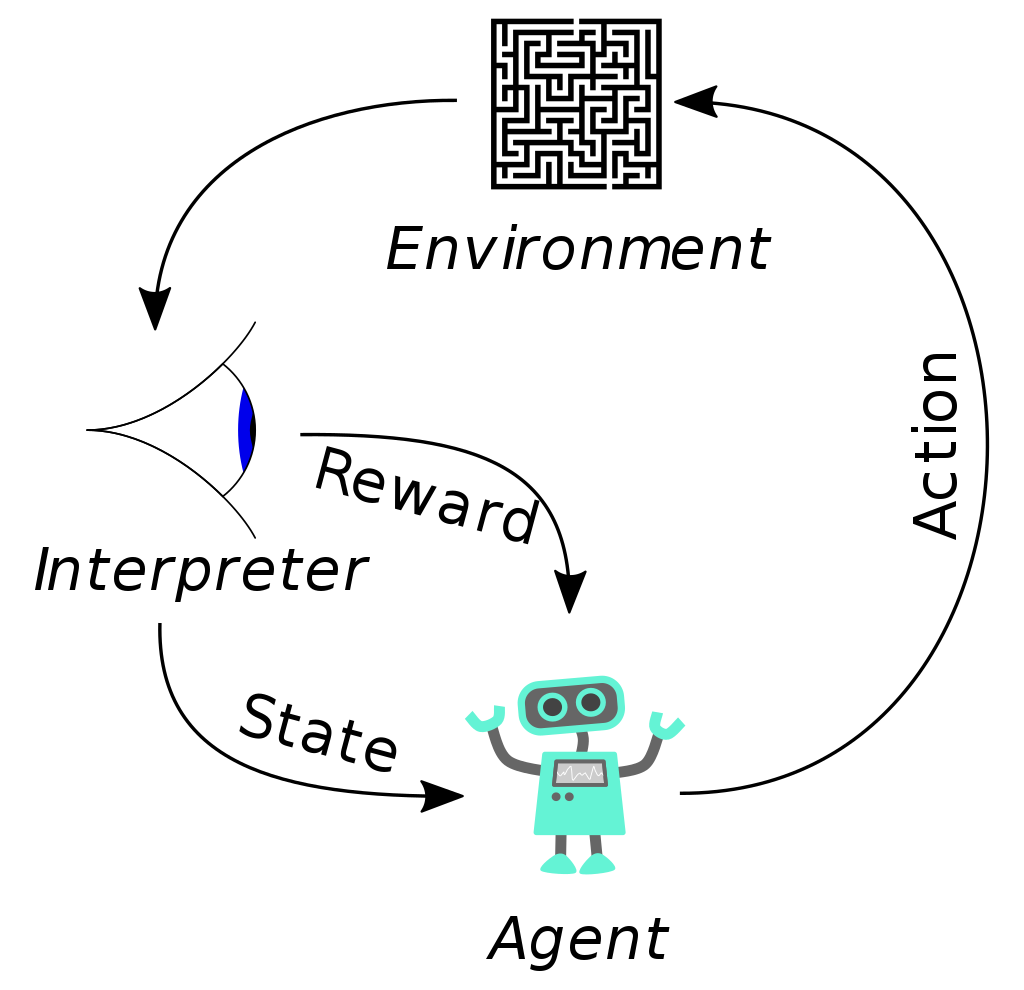
\includegraphics[width=10cm]{assets/rl_diagram.png}
    \caption{Prikaz ciklusa i interakcije agenta s okolinom}
    \label{fig:rl}
\end{figure}

Onaj dio s towards science oko explorationa...


\section{Neuronske mreže}

\subsection{Potpuno povezane neuronske mreže}

\subsection{Konvolucijske neuronske mreže}

\section{Algoritmi podržanog učenja}

\subsection{Deep Q Learning}
\subsection{Double Deep Q Learning}
\subsection{Double Deep Q Learning}

% faza učenja modela, faza iskorištavanja modela